\documentclass[conference]{IEEEtran}
\IEEEoverridecommandlockouts
% The preceding line is only needed to identify funding in the first footnote. If that is unneeded, please comment it out.
\usepackage{cite}
\usepackage{amsmath,amssymb,amsfonts}
\usepackage{algorithmic}
\usepackage{graphicx}
\usepackage{url}
\usepackage[utf8]{inputenc}
\usepackage{textcomp}
\usepackage{multirow}
\usepackage{booktabs}
\usepackage{subfig}
\usepackage{nameref}

\usepackage[english,ngerman,brazilian]{babel}
\def\BibTeX{{\rm B\kern-.05em{\sc i\kern-.025em b}\kern-.08em
    T\kern-.1667em\lower.7ex\hbox{E}\kern-.125emX}}
\begin{document}

\title{PD6 - Rastreamento Visual}

\author{\IEEEauthorblockN{Frederico Guth (18/0081641)}
\IEEEauthorblockA{\textit{Tópicos em Sistemas de Computação, ,} \\
\textit{Turma TC - Visão Computacional (PPGI)}\\
\textit{Universidade de Brasília}\\
Brasília, Brasil\\
fredguth@fredguth.com}
}

\maketitle

\begin{abstract}
Rastreamento visual lida com a localização de objetos em vídeos e tem uma grande variedade de aplicações. Neste projeto, implementamos dois algoritmos para rastrear carros em vídeos de perseguição policial e avaliamos os resultados usando métricas de acurácia e robustez.
\end{abstract}

\begin{IEEEkeywords}
rastreamento de objetos, rastreamento visual, Filtro de Kalman, Rastreador KCF, perseguição policial de carros
\end{IEEEkeywords}

\section{Introdução}

Rastreamento visual lida com a localização de objetos em vídeos e tem uma grande variedade de aplicações: interação homem-computador, vigilância, edição de vídeo, controle de braços mecânicos, entre outras\cite{wikipedia}. 

O rastreamento pode ser 2D, quando o objetivo é seguir a posição na imagem do objeto que se move quadro a quadro, ou 3D, quando se quer usar medidas nas imagens para ajustar com 6 graus de liberdade (3 de translação e 3 de rotação) a posição do objeto no espaço 3D. 

A natureza do problema em que tanto a imagem do objeto alvo, quanto do ambiente onde se encontra,  podem mudar ao longo do tempo e a necessidade de resultados em tempo real, que muitas das aplicações práticas necessitam, tornam esse um problema de grande interesse acadêmico. 

\subsection{Objetivo}
O objetivo deste projeto é rastrear carros em vídeos de perseguição policial e avaliar os resultados usando métricas de sobreposição média e robustez, especificadas em \cite{cehovin}.

\section{Revisão Teórica}

\subsection{Rastreador KCF}
\begin{figure}[ht!]
\begin{center}
\label{kcf-table}
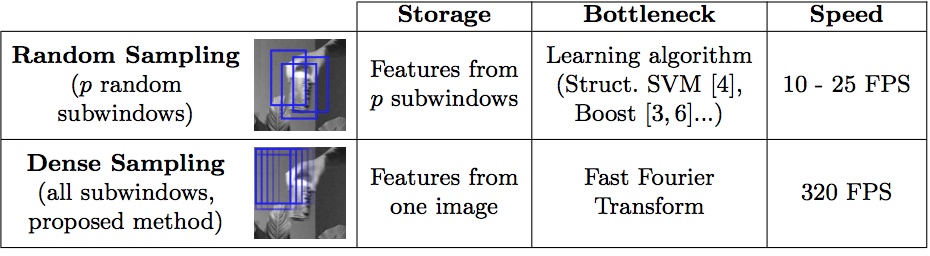
\includegraphics[width=\columnwidth]{tabela-henriques.png}
\caption{Principais diferenças entre técnicas de rastreamento por detecção tradicionais versus KCF. Velocidade para regiões de 64x64 pixels\cite{henriques2012}.}
\end{center}
\end{figure}
Um dos grandes avanços recentes na pesquisa em rastreamento visual foi a adoção de métodos de aprendizado que fazem "rastreamento por detecção". Dado uma amostra da imagem do alvo, o objetivo é que um modelo classificador aprenda a discriminar entre o alvo e o ambiente em uma fase de treinamento. A cada deteção, uma nova imagem do alvo pode ser usada para melhorar o modelo do classificador\cite{henriques, henriques2012}.

Um desafio é o número praticamente ilimitado de possíveis amostras negativas que podem ser retiradas da imagem, que torna tentador focar na caracterização do objeto de interesse\cite{henriques}. Isto é o que acontece na maioria dos algoritmos de rastreamento por detecção. Eles adotam uma estratégia de amostragem esparsa, onde cada amostra é uma \textit{cropagem} da imagem com o tamanho do alvo, com alguma translação e/ou rotação a partir deste\cite{henriques2012}. Como há muita sobreposição entre as amostras, os modelos contém muita redundância (vide figura \ref{kcf-table}) e pouca amostragem de negativos.

A grande contribuição da pesquisa de Henriques \textit{et al} foi constatar que o processo de \textit{cropagem} de imagens levam a uma \textit{matriz circulante}, que pode ser diagonalizada com uma transformada rápida de Fourier (FFT) e que incorpora as informações de todas as potenciais \textit{cropagens}, o que chamam de amostragem densa, sem precisar itera-las com custosos processamentos de matrizes\cite{henriques, henriques2012}.

A regressão linear da formulação que obtiveram é equivalente a um filtro de correlação, usado em diversos outros rastreadores. Mas para regressão por kernel, a formulação obtida, \textit{Kernelized Correlation Filter} (KCF), diferentemente de outras soluções por kernel, tem a mesma complexidade das regressões lineares\cite{henriques}.

O rastreador KCF implementado na OpenCV\cite{opencv} permite uma avaliação do mesmo em termos de acurácia e robustez. É importante registrar, no entanto, que é uma implementação simples com várias oportunidades de melhoria.  Além de uma melhor documentação, a implementação não inclui deteção de falhas do modelo, nem incorpora modelos de incerteza, como por exemplo filtro de Kalman. \label{kcf-opencv}

\subsection{Filtro de Kalman}
\begin{figure}[ht!]
\begin{center}
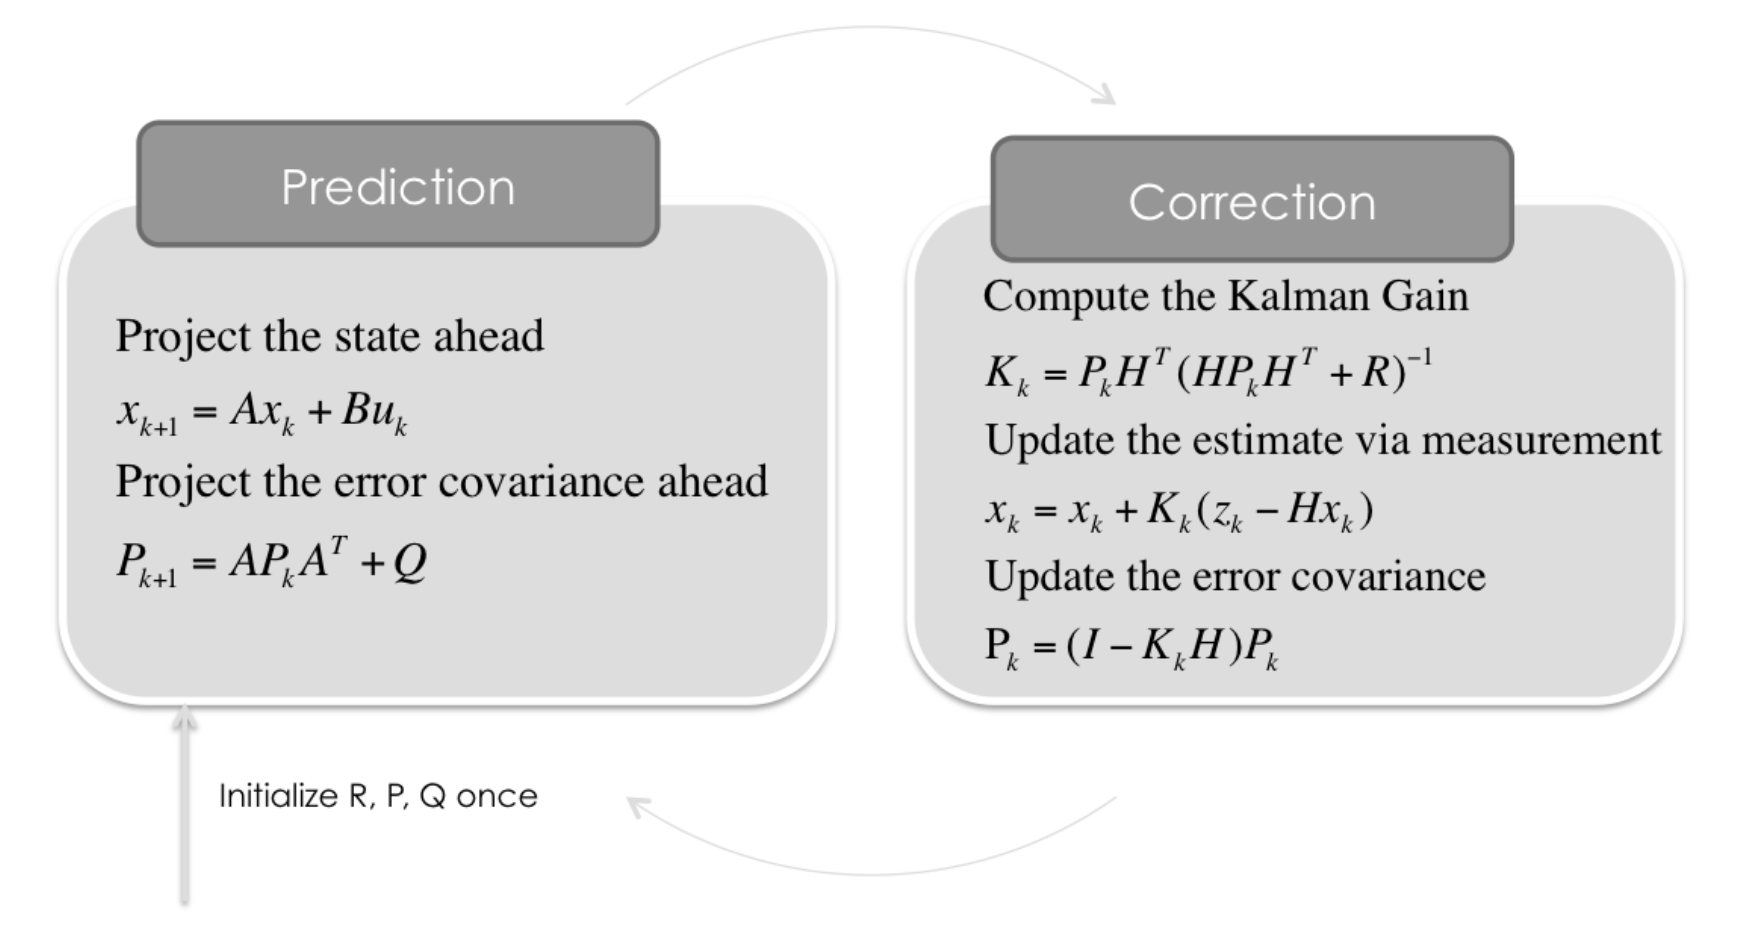
\includegraphics[width=\columnwidth]{kalman.png}
\caption{As duas etapas do filtro de Kalman\cite{balzer82}}
\label{etapas-kalman}
\end{center}
\end{figure}

O filtro de Kalman é um algoritmo que usa uma série de medidas observadas ao longo do tempo, contendo ruído estatístico e outras 
incertezas, e produz estimativas da grandeza medida que tendem a se aproximar mais dos valores reais do que aquelas realizadas a partir de apenas uma medida\cite{wikipedia}. Essa técnica foi primeiramente publicada por Rudolf E. Kalman, em 1960\cite{kalman}, e tem diversas aplicações práticas, principalmente em sistemas de navegação e controle de veículos aéreos e espaciais, tendo inclusive sido amplamente utilizada  no projeto espacial Apollo que colocou o primeiro homem na Lua\cite{grewal}.


O filtro de Kalman tem duas etapas principais: a etapa de predição e a de correção (vide figura \ref{etapas-kalman}). A etapa de predição é responsável por estimar o estado futuro, a partir do estado corrente. A etapa de correção melhora as estimativas futuras, a partir de medidas reais do estado corrente. 


\section{Metodologia}\label{metodologia}

\subsection{Materiais}
Foram utilizados:
\begin{itemize}
\item computador MacBook Pro (Retina, 13-inch, Early 2015), Processador Intel Core i5 2,7 GHz, 8GB de RAM
\item Python 3.6.3 :: Anaconda custom (64-bit)
\item OpenCV 3.4.0
\item 5 programas python e 1 notebook jupyter especialmente desenvolvidos para o projeto. Todos estão disponíveis no repositório: \url{git@github.com:fredguth/unb-cv-3183.git}\label{repo}
\end{itemize}
Todos os arquivos do projeto estão publicamente disponíveis em  \url{git@github.com:fredguth/unb-cv-3183.git}\label{repo}

\subsection{Visão Geral}
Foram implementados dois algoritmos:

 \begin{enumerate}
  \item rastreador KCF; e
  \item  rastreador KCF com filtro de Kalman. 
\end{enumerate}

\subsection{Rastreador KCF}

O rastreador KCF foi desenvolvido (r3.py) usando a implementação disponível na biblioteca OpenCV. 
\begin{enumerate}
  \item executamos o programa r3.py com 2 vídeos de perseguição;
  \item em cada execução, guardamos as métricas obtidas;
\end{enumerate}

\subsection{Rastreador KCF com filtro de Kalman}
Como o algoritmo KCF não inclui um detector de falhas, usamos o filtro de Kalman corrigindo-o com a estimativa do KCF.  Com isso, apenas \textit{amortecemos} o resultado do KCF, e melhoramos sua robustez, pois quando este perde o objeto rastreado, reinicializamos com a estimativa do filtro de Kalman.

Obviamente essa não é a melhor forma de aplicar o filtro de Kalman. O ideal seria desenvolver um detector de falhas para o KCF e ajustar o Kalman a partir deste. Na nossa implementação, \textit{trocamos} acurácia por robustez, o que não seria absolutamente necessário em uma implementação com filtro de Kalman com detecção de falhas. De toda forma, acreditamos que o resultado deste experimento pode nos indicar o potencial benefício de uma nova implementação do KCF que incorpore esses itens.

Por último, é importante mencionar também que a implementação do filtro de Kalman na OpenCV, além de muito mal documentada, não permite inicializar o filtro com um estado inicial, sendo sempre inicializado com uma matriz de zeros, o que nos obriga sempre a somar ou subtrair o estado inicial quando se deseja utilizar as funções de predição e correção do filtro.
\begin{enumerate}
  \item executamos o programa r4.py com 2 vídeos de perseguição;
  \item em cada execução, guardamos as métricas obtidas;
\end{enumerate}

\subsection{Métricas}
  %  \eq \sum_{t}
  %   
  
Para avaliar os rastreadores, usamos duas medidas sugeridas por \cite{cehovin}.


\begin{enumerate}
  \item sobreposição média:
 \begin{equation}
    \overline{\phi} = \sum_{t}\frac{\phi_{t}}{N},
\end{equation}
onde:
\begin{equation}
    \phi_{t} = \frac{R^{G}_{t} \cap R^{T}_{t}}{R^{G}_{t} \cup R^{T}_{t}},
\end{equation} 
sendo $R^{G}_{t}$ a região no \textit{ground-truth}, $R^{T}_{t}$ a região alvo prevista pelo rastreador e N o número de quadros para os quais temos informação (\textit{ground-truth}).
  \item  robustez:
  \begin{equation}
    R_{S} = e^{-S\frac{F_{0}}{N}},
\end{equation}
onde $F_{0}$ é o número de falhas em $N$ quadros e $S$ é um parâmetro que pode ser interpretado como a probabilidade do rastreador continuar funcionando $S$ quadros após a última falha\cite{cehovin}.
No presente projeto, usamos $S=30$.
\end{enumerate}

\subsection{Condições de reiniacialização}
Os rastreadores rodam enquanto $\phi > 0$. Quando a acurácia é zero, uma falha é contabilizada e o rastreador reinicializado com \textit{ground-truth} do quadro.

\section{Resultados}
Nesta seção apresentamos os resultados obtidos. Todos os dados podem ser acessados no repositório do projeto (\ref{repo}).

Quantitativamente, os resultados foram interessantes, como se pode ver na Tabela \ref{tabela}.


\begin{table}[]
\centering
\caption{Média da acurácia e robustez}
\label{tabela}
\begin{tabular}{@{}llll@{}}
\toprule
 & Video & $\overline{\phi}\%$ & $\overline{R}\%$ \\ \midrule
\multicolumn{1}{l}{\multirow{2}{*}{KCF}} & \multicolumn{1}{l}{1} & \multicolumn{1}{l}{84.91} & \multicolumn{1}{l}{56.85} \\ \cmidrule(l){2-4} 
\multicolumn{1}{l}{} & \multicolumn{1}{l}{2} & \multicolumn{1}{l}{77.85} & \multicolumn{1}{l}{41.23} \\ \midrule
\multicolumn{1}{l}{\multirow{2}{*}{Kalman}} & \multicolumn{1}{l}{1} & \multicolumn{1}{l}{83.19} & \multicolumn{1}{l}{92.61} \\ \cmidrule(l){2-4} 
\multicolumn{1}{l}{} & \multicolumn{1}{l}{2} & \multicolumn{1}{l}{68.61} & \multicolumn{1}{l}{78.07} \\ \bottomrule
\end{tabular}
\end{table}

\subsection{Rastreador KCF}
\begin{figure}
\centering
\subfloat[KCF - video 1]{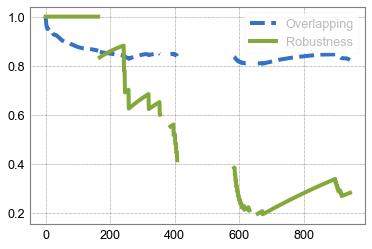
\includegraphics[width=4cm]{car1basic.png}}\hfil
\subfloat[KCF - video 2]{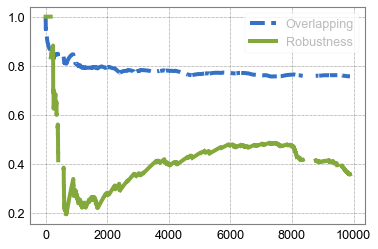
\includegraphics[width=4cm]{car2basic.png}}
\caption{Acurácia e robustez do KCF ao longo do tempo}
\label{kcf}
\end{figure}
Na figura \ref{kcf} podemos ver o comportamento do rastreador KCF nos dois videos ao longo do tempo (quadros).  As falhas nos gráficos apontam as regiões para as quais não temos os valores de \textit{ground-truth}. É interessante notar que, nas duas instâncias, a acurácia logo cai para um patamar acima de 80\% e não piora. A robustez varia bastante e chega a valores bem baixos em ambos os vídeos, próximo a 20\%, mas melhoram até o final.
\subsection{Rastreador Kalman}

\begin{figure}
\centering
\subfloat[Kalman - video 1]{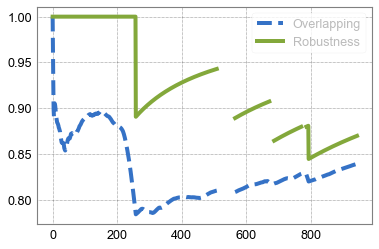
\includegraphics[width=4cm]{car1kalman.png}}\hfil
\subfloat[Kalman - video 2]{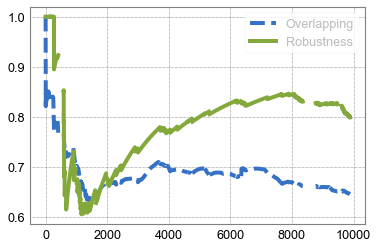
\includegraphics[width=4cm]{car2kalman.png}}
\caption{Acurácia e robustez do Filtro de Kalman ao longo do tempo.}\label{kalman}
\end{figure}

Na figura \ref{kalman} podemos observar o efeito do filtro de Kalman. A acurácia cai bastante nos quadros com mudança de zoom, mas melhora ao longo do tempo. A robustez, entretanto, nunca cai abaixo de 60\%.

\subsection{Análise dos resultados}
Os resultados obtidos foram dentro do esperado. Com filtro de Kalman, \textit{trocamos} acurácia por robustez, entretanto vale ressaltar que no primeiro vídeo, o filtro de Kalman tem uma acurácia apenas 1,1\% pior que o KCF, enquanto a robustez é 62,90\% melhor. No vídeo 2, a acurácia com filtro de Kalman cai 11.87\%, enquanto a robustez melhora 89.35\%. 

Notamos que o \textit{zoom} no vídeo é uma grande fonte de falhas, para minimizar esse problema, uma medida dessa grandeza poderia ser obtida, a partir da largura das faixas dos carros, e incorporada ao filtro de Kalman.

Como já mencionado \ref{kcf-opencv}, o algoritmo KCF implementado na OpenCV não implementa detecção de falhas.  Acreditamos que uma implementação que considere falhas e aplique nessa medida o filtro de Kalman pode ter resultados melhores. 


\section{Discussão e Conclusões}
Neste trabalho, implementamos dois algoritmos para rastreamento visual de objetos em vídeo. O algoritmo KCF apresenta bons resultados de acurácia e robustez.  Entretanto, mostramos que seu modelo pode melhorar se incorporar incerteza, o que pode ser feito com um filtro de Kalman. Ao \textit{amortecer}  o resultado do KCF com um filtro de Kalman, tivemos resultados de robustez entre 60 e 90\% melhores, com perdas de acurácia menores que 12\%, esse resultado serve de inspiração para melhorias na implementação do rastreador KCF da OpenCV. 

% \begin{figure}[htbp]
% \centerline{
\includegraphics{fig.jpg}}
% \caption{Example of a figure caption.}
% \label{fig}
% \end{figure}

\selectlanguage{brazilian}
\bibliographystyle{IEEEtran}
\bibliography{references}

\end{document}
